%----------------------------------------------------------------------------------------
%	PACKAGES AND OTHER DOCUMENT CONFIGURATIONS
%------------------------------------------------------------------------
\documentclass[11pt]{article}

\usepackage[utf8]{inputenc} % Required for inputting international characters
\usepackage[T1]{fontenc} % Output font encoding for international characters
\usepackage{mathpazo} % Palatino font
\usepackage[czech]{babel} % Czech
\usepackage{graphicx}  % Graphics

\begin{document}

%----------------------------------------------------------------------------------------
%	TITLE PAGE
%----------------------------------------------------------------------------------------

\begin{titlepage} % Suppresses displaying the page number on the title page and the subsequent page counts as page 1
	\newcommand{\HRule}{\rule{\linewidth}{0.5mm}} % Defines a new command for horizontal lines, change thickness here
	
	\center % Centre everything on the page
	
	%------------------------------------------------
	%	Headings
	%------------------------------------------------
	
	\textsc{\LARGE České vysoké učení technické v Praze}\\[1.5cm] % Main heading such as the name of your university/college
	
	\textsc{\Large Algoritmy digitální kartografie a GIS}\\[0.5cm] % Major heading such as course name
	
	\textsc{\large Katedra geomatiky}\\[0.5cm] % Minor heading such as course title
	
	%------------------------------------------------
	%	Title
	%------------------------------------------------
	
	\HRule\\[0.4cm]
	
	{\huge\bfseries Úloha č. 1: Geometrické vyhledávání bodu}\\[0.4cm] % Title of your document
	
	\HRule\\[1.5cm]
	
	%------------------------------------------------
	%	Author(s)
	%------------------------------------------------
	
	

	
	% If you don't want a supervisor, uncomment the two lines below and comment the code above
	Monika \textsc{Křížová} % Your name
	
	Marek \textsc{Hoffmann}
	
	%------------------------------------------------
	%	Date
	%------------------------------------------------
	
	\vfill\vfill\vfill % Position the date 3/4 down the remaining page
	
	{\large 18.10.2021} % Date, change the \today to a set date if you want to be precise
	
	%------------------------------------------------
	%	Logo
	%------------------------------------------------
	
	%\vfill\vfill
	%\includegraphics[width=0.2\textwidth]{placeholder.jpg}\\[1cm] % Include a department/university logo - this will require the graphicx package
	 
	%----------------------------------------------------------------------------------------
	
	\vfill % Push the date up 1/4 of the remaining page
	
\end{titlepage}

%----------------------------------------------------------------------------------------


%----------------------------------------------------------------------------------------
%	TABLE OF CONTENT
%----------------------------------------------------------------------------------------

\tableofcontents
%\thispagestyle{empty}

\clearpage

\section{Zadání}

\begin{figure}[htbh]
	\centering
	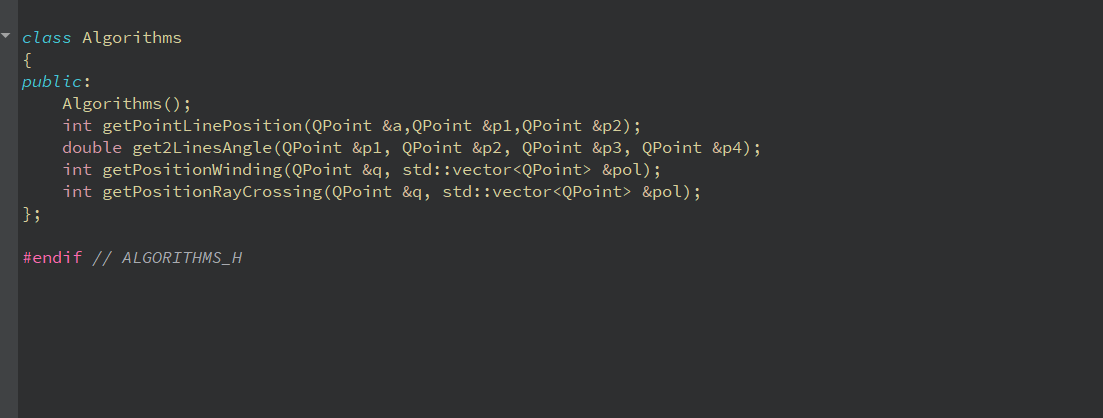
\includegraphics[scale=0.55]{images/appka.png} 
	\caption{Takto vypada nase appka}
	\label{fig:ostruzna_mapa.}
\end{figure} 

\clearpage

\section{Popis a rozbor problému + vzorce.}
\clearpage

\section{Popisy algoritmů formálnímm jazykem.}
\clearpage

\section{Problematické situace a jejich rozbor (tj. simplexy) + ošetření těchto situací v kódu.}
\clearpage

\section{Vstupní data, formát vstupních dat, popis.}
\clearpage

\section{Výstupní data, formát výstupních da, popis.}
\clearpage

\section{Printscreen vytvořené aplikace.}
\clearpage

\section{Dokumentaci: popis tříd, datových položek a jednotlivých metod..}
\clearpage

\section{Závěr, možné či neřešené problémy, náměty na vylepšení.}
\clearpage

\section{Seznam literatury}
\clearpage





\end{document}
